% ŠABLONA PRO PSANÍ ZÁVĚREČNÉ STUDIJNÍ PRÁCE
%%%%%%%%%%%%%%%%%%%%%%%%%%%%%%%%%%%%%%%%%%%%
% Autor: Jakub Dokulil (kubadokulil99@gmail.com)
% Tato šablona byla vytvořena tak, aby pomocí ní mohli v systému LaTeX soutěžící sázet své práce a zároveň odpovídala požadavkům na formátování vyplývajícím z wordové šablony umístěné na webu soc.cz.
%
\documentclass[12pt, a4paper,
%oneside,      %% -- odkomentujte, pokud chcete svou práci mít pouze jednostrannou, mezera pro hřbet pak automaticky bude pouze na levé straně
twoside,        %% -- pro oboustranné práce, mezera pro hřbet následně střídá strany.
openright
]{report}

%% Nutné balíčky a nastavení
%%%%%%%%%%%%%%%%%%%%%%%%%%%%

%% Proměnné
\newcommand\obor{INFORMAČNÍ TECHNOLOGIE} %% -- napiš číslo a název tvého oboru
\newcommand\kodOboru{18-20-M/01} %% -- napiš číslo a název tvého oboru
\newcommand\zamereni{se zaměřením na počítačové sítě a programování} %% -- napiš číslo a název tvého oboru
\newcommand\skola{Střední škola průmyslová a umělecká, Opava} %% vyplň název školy
\newcommand\trida{IT4} %% vyplň jméno svého konzultanta
\newcommand\jmenoAutora{Daniel Antoš}  %% vyplň své jméno
\newcommand\skolniRok{2023/24} %% vyplň rok
\newcommand\datumOdevzdani{1. 1. 2024} %% vyplň rok
\newcommand\nazevPrace{Programovací jazyk Ruda} %% vyplň název své práce

\title{\nazevPrace} %% -- Název tvé práce
\author{\jmenoAutora} %% -- tvé jméno
\date{\datumOdevzdani} %% -- rok, kdy píšeš SOČku

\usepackage[top=2.5cm, bottom=2.5cm, left=3.5cm, right=1.5cm]{geometry} %% nastaví okraje, left -- vnitřní okraj, right -- vnější okraj

\usepackage[czech]{babel} %% balík babel pro sazbu v češtině
\usepackage[utf8]{inputenc} %% balíky pro kódování textu
\usepackage[T1]{fontenc}
\usepackage{cmap} %% balíček zajišťující, že vytvořené PDF bude prohledávatelné a kopírovatelné

\usepackage{graphicx} %% balík pro vkládání obrázků

\usepackage{subcaption} %% balíček pro vkládání podobrázků

\usepackage{hyperref} %% balíček, který v PDF vytváří odkazy

\linespread{1.25} %% řádkování
\setlength{\parskip}{0.5em} %% odsazení mezi odstavci


\usepackage[pagestyles]{titlesec} %% balíček pro úpravu stylu kapitol a sekcí
\titleformat{\chapter}[block]{\scshape\bfseries\LARGE}{\thechapter}{10pt}{\vspace{0pt}}[\vspace{-22pt}]
\titleformat{\section}[block]{\scshape\bfseries\Large}{\thesection}{10pt}{\vspace{0pt}}
\titleformat{\subsection}[block]{\bfseries\large}{\thesubsection}{10pt}{\vspace{0pt}}


\usepackage{tocloft} % Balíček umožní přizpůsobit vzhled tabulky obsahu
\setlength{\cftbeforechapskip}{0pt}  % Menší rozestup pro kapitoly
\setlength{\cftbeforesecskip}{0pt}   % Menší rozestup pro sekce

\setcounter{secnumdepth}{2}
\setcounter{tocdepth}{1}
\usepackage{fancyhdr}
\pagestyle{fancy}
\fancyhf{}
\renewcommand{\headrulewidth}{0pt}
\fancyfoot[C]{\thepage}

\usepackage{booktabs}

\usepackage{url}

%% Balíčky co se můžou hodit :) 
%%%%%%%%%%%%%%%%%%%%%%%%%%%%%%%

\usepackage{pdfpages} %% Balíček umožňující vkládat stránky z PDF souborů, 

\usepackage{upgreek} %% Balíček pro sazbu stojatých řeckých písmen, třeba u jednotky mikrometr. Například stojaté mí: \upmu, stojaté pí: \uppi

\usepackage{amsmath}    %% Balíčky amsmath a amsfonts 
\usepackage{amsfonts}   %% pro sazbu matematických symbolů
\usepackage{esint}     %% pro sazbu různých integrálů (např \oiint)
\usepackage{mathrsfs}
\usepackage{helvet} % Helvet font
\usepackage{mathptmx} % Times New Roman
\usepackage{Oswald} % Oswald font


%% makra pro sazbu matematiky
\newcommand{\dif}{\mathrm{d}} %% makro pro sazbu diferenciálu, místo toho
%% abych musel psát '\mathrm{d}' mi stačí napsat '\dif' což je mnohem 
%% kratší a mohu si tak usnadnit práci

\let\oldchapter\chapter
\renewcommand{\chapter}{
	\clearpage
	\pagestyle{fancy}
	\oldchapter
}

\renewcommand\bibname{Seznam použitých zdrojů}


\usepackage{listings}
\usepackage{xcolor}

\renewcommand{\lstlistingname}{Kód}% Listing -> Algorithm
\renewcommand{\lstlistlistingname}{Seznam programových kódů}% List of Listings -> List of Algorithms

%% Definice 
\lstdefinelanguage{JavaScript}{
	morekeywords=[1]{break, continue, delete, else, for, function, if, in,
		new, return, this, typeof, var, void, while, with},
	% Literals, primitive types, and reference types.
	morekeywords=[2]{false, null, true, boolean, number, undefined,
		Array, Boolean, Date, Math, Number, String, Object},
	% Built-ins.
	morekeywords=[3]{eval, parseInt, parseFloat, escape, unescape},
	sensitive,
	morecomment=[s]{/*}{*/},
	morecomment=[l]//,
	morecomment=[s]{/**}{*/}, % JavaDoc style comments
	morestring=[b]',
	morestring=[b]"
}[keywords, comments, strings]


\lstdefinelanguage[ECMAScript2015]{JavaScript}[]{JavaScript}{
	morekeywords=[1]{await, async, case, catch, class, const, default, do,
		enum, export, extends, finally, from, implements, import, instanceof,
		let, static, super, switch, throw, try},
	morestring=[b]` % Interpolation strings.
}

\lstalias[]{ES6}[ECMAScript2015]{JavaScript}

% Nastavení barev
% Requires package: color.
\definecolor{mediumgray}{rgb}{0.3, 0.4, 0.4}
\definecolor{mediumblue}{rgb}{0.0, 0.0, 0.8}
\definecolor{forestgreen}{rgb}{0.13, 0.55, 0.13}
\definecolor{darkviolet}{rgb}{0.58, 0.0, 0.83}
\definecolor{royalblue}{rgb}{0.25, 0.41, 0.88}
\definecolor{crimson}{rgb}{0.86, 0.8, 0.24}

% Nastavení pro Python
\lstdefinestyle{Python}{
	language=Python,
	backgroundcolor=\color{white},
	basicstyle=\ttfamily,
	breakatwhitespace=false,
	breaklines=false,
	captionpos=b,
	columns=fullflexible,
	commentstyle=\color{mediumgray}\upshape,
	emph={},
	emphstyle=\color{crimson},
	extendedchars=true,  % requires inputenc
	fontadjust=true,
	frame=single,
	identifierstyle=\color{black},
	keepspaces=true,
	keywordstyle=\color{mediumblue},
	keywordstyle={[2]\color{darkviolet}},
	keywordstyle={[3]\color{royalblue}},
	literate=%
	{á}{{\'a}}1 {č}{{\v{c}}}1 {ď}{{\v{d}}}1 {é}{{\'e}}1 {ě}{{\v{e}}}1
	{í}{{\'i}}1 {ň}{{\v{n}}}1 {ó}{{\'o}}1 {ř}{{\v{r}}}1 {š}{{\v{s}}}1
	{ť}{{\v{t}}}1 {ú}{{\'u}}1 {ů}{{\r{u}}}1 {ý}{{\'y}}1 {ž}{{\v{z}}}1,		
	numbers=left,
	numbersep=5pt,
	numberstyle=\tiny\color{black},
	rulecolor=\color{black},
	showlines=true,
	showspaces=false,
	showstringspaces=false,
	showtabs=false,
	stringstyle=\color{forestgreen},
	tabsize=2,
	title=\lstname,
	upquote=true  % requires textcomp	
}


\lstdefinestyle{JSES6Base}{
	backgroundcolor=\color{white},
	basicstyle=\ttfamily,
	breakatwhitespace=false,
	breaklines=false,
	captionpos=b,
	columns=fullflexible,
	commentstyle=\color{mediumgray}\upshape,
	emph={},
	emphstyle=\color{crimson},
	extendedchars=true,  % requires inputenc
	fontadjust=true,
	frame=single,
	identifierstyle=\color{black},
	keepspaces=true,
	keywordstyle=\color{mediumblue},
	keywordstyle={[2]\color{darkviolet}},
	keywordstyle={[3]\color{royalblue}},
 literate=%
{á}{{\'a}}1 {č}{{\v{c}}}1 {ď}{{\v{d}}}1 {é}{{\'e}}1 {ě}{{\v{e}}}1
{í}{{\'i}}1 {ň}{{\v{n}}}1 {ó}{{\'o}}1 {ř}{{\v{r}}}1 {š}{{\v{s}}}1
{ť}{{\v{t}}}1 {ú}{{\'u}}1 {ů}{{\r{u}}}1 {ý}{{\'y}}1 {ž}{{\v{z}}}1,		
	numbers=left,
	numbersep=5pt,
	numberstyle=\tiny\color{black},
	rulecolor=\color{black},
	showlines=true,
	showspaces=false,
	showstringspaces=false,
	showtabs=false,
	stringstyle=\color{forestgreen},
	tabsize=2,
	title=\lstname,
	upquote=true  % requires textcomp
}

\lstdefinestyle{JavaScript}{
	language=JavaScript,
	style=JSES6Base,
}
\lstdefinestyle{ES6}{
	language=ES6,
	style=JSES6Base
}


%% Bordel pro práci - můžeš smáznout :) 
%%%%%%%%%%%%%%%%%%%

\usepackage{lipsum} %% balíček který píše lipsum (nesmyslný text, který se používá pro kontrolu typografie)

%% Začátek dokumentu
%%%%%%%%%%%%%%%%%%%%
\begin{document}
	
	\pagestyle{empty}
	\pagenumbering{Roman}
	
	\clearpage

%% Titulní stránka s informacemi
%%%%%%%%%%%%%%%%%%%%%%%%%%%%%%%%%%%%%%%%
	
	{\fontfamily{phv}\selectfont
		%% Logo školy
		\begin{figure}[h]
			\centering
			
\includegraphics[width=0.6\linewidth]{image/logo-skoly.png} 
		\end{figure}
		
		
		%% Hlavička práce a její název (viz proměnná \nazev prace)
		%% \sffamily %%% bezpatkové písmo - sans serif
		{\bfseries %%% písmo na stránce je tučně
			\begin{center}
				\vspace{0.025 \textheight}
				\LARGE{ZÁVĚREČNÁ STUDIJNÍ PRÁCE}\\
				\large{dokumentace}\\
				\vspace{0.075 \textheight}
				\LARGE {\nazevPrace}\\
			\end{center}  
		}%%%
		
		\begin{figure}[h]
			\centering
			
\includegraphics[width=0.5\linewidth]{image/logo.png} 
		\end{figure}
		
		\vspace{0.02 \textheight}
		\begin{table}[h!]
			\begin{tabular}{ll}
				\textbf{Autor:} & \jmenoAutora\\ 
				\textbf{Obor:} & \kodOboru { } \obor\\
				\textbf{} & \zamereni\\
				\textbf{Třída:} & \trida\\
				\textbf{Školní rok:} & \skolniRok\\
			\end{tabular}
			
		\end{table}		
	}
	
	


%% Prohlášení - povinné
%%%%%%%%%%%%%%%%%%%%%%%%%%%%
	\vspace*{0.7\textheight} %% Vertikální mezeru je možné upravit
	\noindent{\large{\bfseries{Prohlášení}\\}}  %% uprav si koncovky podle toho na jaký rod se cítíš, vypadá to pak lépe :) 
	\noindent{Prohlašuji, že jsem závěrečnou práci vypracoval samostatně a uvedl veškeré použité 
		informační zdroje.\\}
	\noindent{Souhlasím, aby tato studijní práce byla použita k výukovým a prezentačním účelům na Střední průmyslové a umělecké škole v Opavě, Praskova 399/8.}
	\vfill
	\noindent{V Opavě \datumOdevzdani\\}
	\noindent
	\begin{minipage}{\linewidth}
		\hspace{9.5cm} 
		\begin{tabular}{@{}p{6cm}@{}}
			\dotfill \\
			Podpis autora
		\end{tabular}
	\end{minipage}
	
	\clearpage %% Zalomení dvojstránky

%% Stránka obsahující abstrakt (anotaci)
%%%%%%%%%%%%%%%%%%%%%%%%%%%%%%%%%%%%%%%%%%%%%%%%%%%%%%%%	

%% Abstrakt v češtině
%%%%%%%%%%%%%%%%%%%%%%%%%%%%
	\noindent{\Large{\bfseries{Abstrakt}\\}}
	\noindent 
	Ruda je programovací jazyk zaměřený na rychlé a snadné prototypování aplikací, umožňující vývojářům rychle testovat nápady bez zbytečné složitosti. Kompiluje se do systémově nezávislého binárního formátu pro rychlé spuštění pomocí Ruda VM. Jednoduchá syntaxe a vestavěné nástroje usnadňují vytváření prototypů. Důraz je kladen na fázi prototypování, s možností přechodu k jinému jazyku či platformě pro finální implementaci. Ruda poskytuje efektivní prostředky pro zkušební vývoj a validaci nápadů před případným přesunem do robustnějšího softwarového prostředí.
	
	\vspace{18pt}
	
	\noindent{\large{\bfseries{Klíčová slova}}}
	
	\noindent Jazyk, kompilace, binární formát
	
	\vspace{18pt}
	
	\clearpage


%% Stránka s generovaným obsahem
%%%%%%%%%%%%%%%%%%%%%%%%%%%%%%%%%%%%%%%	
	
	\tableofcontents %% Vygeneruje tabulku s obsahem

	\pagenumbering{arabic} %% Nastavení způsobu číslování stránek (alternativy roman | Roman)
	\setcounter{page}{1} %% Nastavení počitadla stránek
	
	\clearpage

%% Stránka s úvodem - povinná část
%%%%%%%%%%%%%%%%%%%%%%%%%%%%%%%%%%%%%%%		
	\chapter*{Úvod}
%Tento příkaz vytvoří novou kapitolu s názvem "Úvod" ve vašem dokumentu.
%Hvězdička * u příkazu \chapter* znamená, že tato kapitola nebude mít číslo. Ve výsledném dokumentu se tedy objeví jako "Úvod" bez předcházejícího čísla kapitoly, které se obvykle zobrazuje u číslovaných kapitol.
%Tento příkaz také znamená, že kapitola se automaticky neobjeví v obsahu, protože LaTeX standardně zahrnuje do obsahu pouze číslované kapitoly.
	\addcontentsline{toc}{chapter}{Úvod}
%Tento příkaz ručně přidává záznam do obsahu.
%První parametr toc označuje, že přidáváme záznam do Table of Contents (obsahu).
%Druhý parametr chapter specifikuje úroveň záznamu. V tomto případě říkáme, že přidávaný záznam má být považován za kapitolu.
%Třetí parametr Úvod je text, který se objeví v obsahu. V tomto případě bude v obsahu zobrazen název "Úvod".	
Ruda je programovací jazyk, který si dává za úkol zjednodušit prvotní fázi vývoje, což je v současnosti mnohdy rezervováno pouze pro omezený počet jazyků. Tyto jazyky ale často vyžadují nástroje třetích stran pro složitější úkoly. Toto se stává problematické zejména pro méně zkušené vývojáře, kteří tak mohou ztratit spustu času výzkumem, nutným k použití knihovny, kterou už nikdy nebudou potřebovat. 

Také stojí za zmínku, že vše, co Ruda obsahuje bylo naprogramované mnou, s výjimkou knihovny SFML pro použití oken, knihovny git2 pro práci s verzovacím systémem git a několika menších knihoven pro utility jako například Toml serializace, hashování a parsování terminálových parametrů.

\noindent
K tomu, abych vyřešil tyto problémy jsem pro Rudu zadal několik cílů:
\begin{itemize}
	\item Vestavěný správce projektu - jeden správce by měl vystačit pro celý projekt.
	\item Garbage collector - oproti ostatním metodám úklidu paměti nevyžaduje téměř žádnou pozornost vývojáře.
	\item Grafické programování - modul pro kreslení na okno zabudovaný přímo do standardní knihovny.
\end{itemize}

\noindent 
V následujících kapitolách podrobně rozeberu proces kompilace zdrojových souborů, včetně jeho parsování. Nastíním strukturu Ruda bytecode a popíšu interpretaci v rámci virtuálního prostředí. Další témata zahrnují vestavěné nástroje, řešení chyb a praktické příklady použití.

%Tipy k psaní úvodu
%Je povinný, nadpis neměňte, rozsah - max. 1 strana. 
%Tato část práce obsahuje: 
%* náhled do řešené problematiky, zdůvodnění volby problematiky, 
%* předem definované cíle práce, 
%* motivaci pro další čtení textu včetně stručného uvedení obsahu následujících kapitol 


\chapter{Programovací jazyk Ruda}

\section{Pozadí vzniku}

\section{Porovnání alternativ}

\chapter{Překladač}

Zdaleka nejrozsáhlejší část celého projektu je právě překladač. Každý jazyk musí projít nějakou formou překladu zdrojového kódu do formy, která je lépe pochopitelná pro počítač. Nejčastější metody jsou kompilace a interpretace. Ruda používá oba tyto způsoby tak, že zdrojový kód na počítači vývojáře projde kompilací a výsledný soubor obsahuje bytecode, který si potom může spustit klient pomocí interpretu Ruda VM.

Proces překladu se nazívá „compiler pipeline,“ při čemž projde kód několika navazujícími transformacemi, kde každá přibližuje kód více k finálnímu produktu.

\section{Analýza}

Při analýze má překladač za úkol pochopit strukturu a fungování zdrojového kódu. A připravuje informace nutné, pro vytvoření výsledného bytecode.

\subsection{Lexikální}

Lexer, jinak řečeno tokenizer, tvoří první část analýzy zdrojového souboru. Hledá nejmenší významové prvky kódu, tzv. tokeny. Ty můžou být například slova, speciální znaky či „bílé znaky“.

I přestože zpracování tokenů není starost lexeru, moje implementace využívá pro tokenizaci 2 kroky. První krok vytvoří „atomické prvky.“ Neprovádí přítom žádnou logiku a pouze zapisuje, co vidí. Druhý krok poté očistí bílé znaky a vytvoří složené tokeny, jako například řetězce a čísla.

\begin{figure}[h]
	\centering
	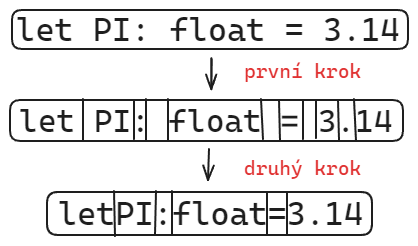
\includegraphics[width=0.5\linewidth]{image/lexer.png}
\end{figure}

\subsection{Syntaktická}

Při syntaktické analýze dochází k parsování vstupních tokenů, hovoříme tak o parseru. Ten postupně prochází tokeny a vytváří z nich strukturu, určenou ke zpracování logickou částí.

Pro Rudu jsem vytvořil vlastní univerzální parser. Používá programovatelný syntax čtený ze souboru, chybová hlášení generuje automaticky, a k tomu nabízí funkce pro debugování pravidel a jednoduchou validaci. Jeho syntax je jednoduchý a přehledný, programátor by měl být schopný zorientovat se už po pár minutách. Klíčové slovo let by v něm mohlo vypadat následovně:

\begin{lstlisting}[numbers=left, caption={Ukázka klíčového slova let}]
KWLet ident type expr
	"let" harderr="true"
	"'text" set="ident"
	: ?
		type ? set="type"
	= ?
		expr ? set="expr"
	; ?;
\end{lstlisting}

První řádek je hlavička slova začínající názvem „KWLet“ a pokračuje jeho parametry. Druhý porovnává, jestli je typ momentálního tokenu text s výrazem „let.“ Pokud ne, vrací error. Pokud ano, pokračuje dál a zapne harderr, ten říká, že pokud odteď dojde k chybě, tak není chybové pouze toto slovo, ale i jeho rodič, který dané slovo porovnával. Dále na řádku 3 porovnává jakýkoliv token reprezentující text. Pokud dojde ke schodě, nastaví parametr ident na porovnávaný token. Pokud nikoliv, vyhodí těžkou chybu (protože je zapnutý harderr). Otazník na řádku 4 znamená, že token není nutný. Pokud bude přítomen, vykoná se kód s vyšším odsazením (řádek č. 5). Středník na konci řádku 8 pouze oznamuje konec definice slova. Vytvořené slovo se později použije stejně jako na řádcích 5 a 7.

Za zmínku stojí také metoda připojení zdrojových souborů. Kompilátor nemůže jen tak zpracovat všechny soubory s příponou .rd, co vidí. To by bylo náročné na zdroje počítače. Tento problém řeší tak, že nejprve získá vstupní soubor (mometálně pouze main.rd). Ten zpracuje a zapíše si použití klíčového slova import, které má cestu k použitému zdroji. Zatím si je pouze zapíše, protože kdyby je ihned zpracoval, tak může dojít k zamrznutí, při použití cyklických importů. Poté je zpracuje a označí jako zpracované.

\cleardoublepage


\subsection{Sémantická}

Poslední fáze analýzy má za úkol dát smysl struktuře získané po parsování. Protože parser je dynamický, tak musí nejprve vše vytáhnout do ucelené podoby a provést případné validace. Kontroluje například zda se neopakují názvy, ale také vytváří typy, parsuje matematické výrazy, apod.


\section{Generace bytecode}

Generace je nejdůležitější část každého překladače. Jde o proces, kdy zpracuje všechna získaná data a vytvoří užitečný produkt v podobě programu, či knihovny.

Má implementace obsahuje generaci nejen bytecode, ale i informací pro debugování. To je užitečné v případě, že běžící Ruda program narazí na problém. Ruda VM díky toho zvládne podat důležité informace o původu problému.

\subsection{Generace}

Překladač před generací prošel třemi fázemi analýzi, aby měl znalost celého kódu. Samotná generace je ale stále velmi náročný proces. V kódu je obrovské množství způsobů, jak přistupovat k datům a jejich manipulaci. Transformace jazyk -> bytecode se potom stává velmi složitá, zmatečná a pokud provedení není perfektní, vytváří prostor pro nečekané chyby.

Překladač začíná tím, že všem funkcím rozdá unikátní ID, které bude velmi důležité později. Vytvoří potřebné objekty společně s Ruda VM (pouze pro kompatibilitu; nikdy ho nespustí). Až bude vše připravené, začne s generací funkcí. Nezáleží na jejich pořadí, nakonec je zpracuje všechny.

Pro překlad funkce používá rekurzivní prohledávání uzlů, které reprezentují výrazy. Pro každý vygeneruje patřičný bytecode. Například pro klíčové slovo let:

\begin{lstlisting}[numbers=left, caption={Překlad klíčového slova let}]
// vyraz
let a = new 60

// bytecode
ReadConst(const_int_60, GENERAL_REG1)
AllocateStatic(1)     
WritePtr(GENERAL_REG1)   
Write(a_stack_pos, POINTER_REG)  
\end{lstlisting}

Výraz vytvoří proměnnou a, do které zapíše ukazatel na hodnotu 60, která je uložená na haldě. Bytecode nejprve přečte hodnotu 60 z paměti a uloží ji do registru GENERAL-REG0. Potom na haldě vytvoří místo pro jednu hodnotu a ukazatel se automaticky uloží do registru POINTER-REG, který potom využije instrukce WritePtr, k tomu, aby na něj zapsala hodnotu z GENERAL-REG1, která je stále číslo 60. Už jenom potřebuje zapsat ukazatel, který stále přebývá v POINTER-REG do pozice na stacku vyhrazené pro proměnnou a.

Tím tenhle příklad končí, ale je nutné vědět, že takhle bude bytecode vypadat až po optimalizaci. Generátor kódu je sám o sobě hloupí a nestará se o žádné stavy. Vždy zohledňuje pouze nejhorší možný případ a vytváří přitom poměrně nekvalitní a hlavně pomalý kód.

\subsection{Optimalizace}

\chapter{Virtuální stroj}

V minulé kapitole jsme prošli, jak ze zdrojového kódu vznikne program. Zde se zaměříme na jeho spuštění pomocí Ruda VM, který je zodpovědný za provedení Ruda programů.

\section{Vlastnosti}

\subsection{Instrukce}

Instrukce jsou jedna ze částí Ruda bytecode. Jde o jednoduché pokyny, popisující co má provést Ruda VM. Jednotlivé instrukce jsou navrhnuté, pro co nejširší možné využití v rámci uzavřeného runtimu. 

Právě proto lze Rudu použít tam, kde je bezpečnost priorita, pokud se povolí pouze moduly standardní knihovny pracující nezávisle na systému. Díky této vlastnosti by v budoucnu mohla Ruda běžet například na serverech, nebo jako skriptovací jazyk v jiném programu.

Pro referenci jednotlivých instrukcí doporučuji prohlédnout přímo zdrojový kód runtimu, který lze nalézt na https://github.com/it-2001/Ruda/blob/main/vm/runtime/src/lib.rs. Zde můžete vyhledat "enum Instructions" (okolo řádku 2500), kde jsou všechny instrukce popsané.

\subsection{Běh programu}

Samotné jádro Rudy je pouze knihovna, nelze tudíž spustit přímo. K tomu pomáhá program Ruda VM, který zpracuje bytecode a připraví podle něj příslušné prostředí pro běh. Kromě toho podává zprávy o stavu, parsuje vstupní argumenty a připravuje potřebné knihovny.

Poté, co Ruda VM připraví vše nutné, tak teprve spustí Ruda program. Instrukce běží sériově, dokud nenarazí na problém, nebo konec programu označený instrukcí End.

\subsection{Model paměti}

\lipsum[80]

\begin{figure}[h]
	\centering
	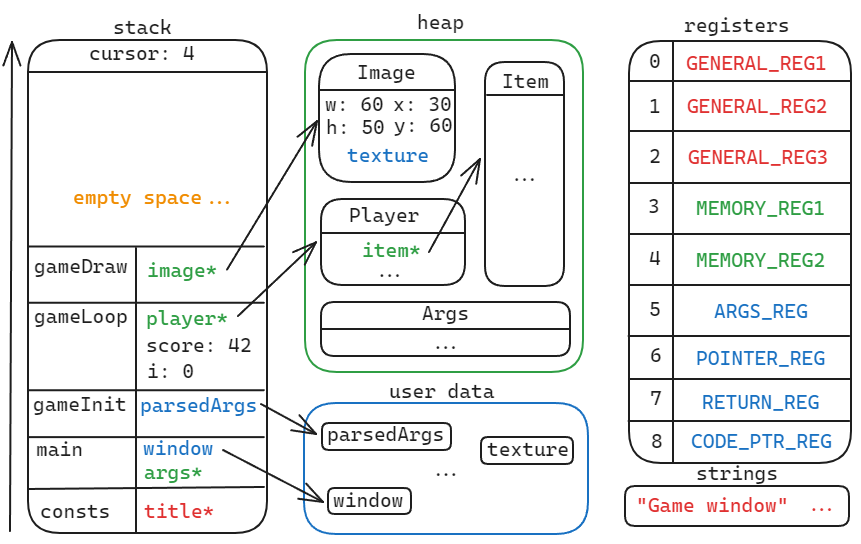
\includegraphics[width=0.8\linewidth]{image/memory.png}
\end{figure}

\section{Garbage collector}

\section{Rozšíření pomocí dynamických knihoven}

\section{Schopnost skriptování}

\chapter{Nástroje pro práci s jazykem}

\section{Dokumentace}

\section{Package manager}

\section{Standardní knihovna}

\section{Grafický inspektor Ruda projektu}

\section{Syntax highlighting}

\chapter{Instalace}

\section{Podporované platformy}

\section{Stažení}

\subsection{Kompilace ze zdrojových kódů}

\subsection{Stažení předkompilované verze}

\section{Proměnné prostředí}

\section{Možné problémy}

\chapter{Programování v Rudě}

\section{Syntaxe}

\section{Příklady}

\chapter{Zhodnocení}

\section{Splněné cíle}

\section{Poznatky}

\section{Možnosti dalšího vývoje}




	
	%% literatura
	\begin{thebibliography}{99}
		\bibitem{sablonaSOC} DOKULIL Jakub. \textit{Šablona pro psaní SOČ v programu \LaTeX} [Online]. Brno, 2020 [cit. 2020-08-24]. Dostupné z: \url{https://github.com/Kubiczek36/SOC_sablona}
		\bibitem{LaTeXprirucka}OETIKER, Tobias, Hubert PARTL, Irene HYNA, Elisabeth SCHEGL, Michal KOČER a Pavel SÝKORA. \textit{Ne příliš stručný úvod do systému LaTeX2e} [online]. 1998 [cit. 2020-08-24]. Dostupné z: \url{https://www.jaroska.cz/elearning/informatika/typografie/lshort2e-cz.pdf}
		\bibitem{wikibooksLaTeX}\textit{Wikibooks: LaTeX} [online]. San Francisco (CA): Wikimedia Foundation, 2001- [cit. 2020-08-24]. Dostupné z: \url{https://en.wikibooks.org/wiki/LaTeX}
		\bibitem{stackExchange} \textit{TeX - LaTeX Stack Exchange} [online]. Stack Exchange, 2020 [cit. 2020-09-01]. Dostupné z: \url{https://tex.stackexchange.com}
		\bibitem{sspuLogo} \textit{Střední škola průmyslová a umělecká Opava} [online]. [cit. 2023-11-11]. Dostupné z: \url{https://www.sspu-opava.cz}
		\bibitem{citacePRO}\textit{Citace PRO} [online]. Citace.com, 2020 [cit. 2020-08-31]. Dostupné z: \url{https://www.citacepro.com}
		\bibitem{Born2019} BORN, Max a Emil WOLF. \textit{Principles of optics: electromagnetic theory of propagation, interference and diffraction of light}. 7th (expanded) edition. Reprinted wirth corrections 2002. 15th printing 2019. Cambridge: Cambridge University Press, 2019. ISBN 978-0-521-64222-4.
	\end{thebibliography}
	
	%% obrázky 
	\listoffigures
	
	%% tabulky
	\listoftables
	
	\appendix %% začínají přílohy
	
	\titleformat{\chapter}[block]{\scshape\bfseries\LARGE}{Příloha \thechapter}{10pt}{\vspace{0pt}}[\vspace{-22pt}] %% nastavení nadpisu u příloh
	

	
	
\end{document}
